\documentclass[10pt]{article}
%\documentclass{amsart}

\usepackage[scaled]{helvet}\renewcommand*\familydefault{\sfdefault}\usepackage[T1]{fontenc}
\usepackage{setspace}\onehalfspacing
\usepackage{fancyhdr}
\pagestyle{fancy}
\renewcommand{\headrulewidth}{0.5pt}
\renewcommand{\footrulewidth}{0.5pt}
\fancyhead[L]{\leftmark}
\fancyhead[R]{}


\usepackage{amsmath}
\usepackage{amsfonts}
\usepackage{IEEEtrantools}
\usepackage{algorithmic}
\usepackage{algorithm}
\usepackage{subfig}

\usepackage{natbib}

\usepackage{tikz}
\usepackage{pgfplots}
 \usetikzlibrary{plotmarks}
 \pgfplotsset{compat=newest}
 \pgfplotsset{plot coordinates/math parser=false}
 \usepgfplotslibrary{external}
 \tikzexternalize[prefix=tikz/]


\newenvironment{meta}[0]{\color{red} \em}{}


\title{Particle Gibbs with Refreshed Backward Simulation}
\author{Pete Bunch and Fredrik Lindsten}
\date{August 2014}

%%% MACROS %%%
\newcommand{\ti}{t}
\newcommand{\timax}{T}

\newcommand{\pr}{\theta}
\newcommand{\prspace}{\Theta}

\newcommand{\ls}[1]{x_{#1}}
\newcommand{\lsspace}{\mathcal{X}}

\newcommand{\ob}[1]{y_{#1}}
\newcommand{\obspace}{\mathcal{Y}}

\newcommand{\nc}{Z}

\newcommand{\toas}{\stackrel{\text{a.s.}}{\to}}
\newcommand{\testfunc}{\zeta}
\newcommand{\prob}{P}

\newcommand{\id}[1]{q_{#1}}

\newcommand{\an}[1]{a_{#1}}
\newcommand{\ai}[1]{b_{#1}}
\newcommand{\notai}[1]{-b_{#1}}
\newcommand{\aifinal}{K}
\newcommand{\lsset}[1]{\mathbf{x}_{#1}}
\newcommand{\anset}[1]{\mathbf{a}_{#1}}

\newcommand{\den}{p}
\newcommand{\ed}{\pi}
\newcommand{\td}[1]{f_{\theta,#1}}
\newcommand{\od}[1]{g_{\theta,#1}}
\newcommand{\pd}[1]{\phi_{#1}}
\newcommand{\spd}[1]{\psi_{#1}}

\newcommand{\pw}[1]{w_{#1}}
\newcommand{\ppw}[1]{v_{#1}}
\newcommand{\spw}[1]{u_{#1}}

\newcommand{\mhap}{\alpha}
\newcommand{\pss}[1]{^{(#1)}}
\newcommand{\nump}{N}
\newcommand{\utf}[1]{\rho_{#1}}
\newcommand{\cised}{\eta}
\newcommand{\cisi}{c}
\newcommand{\notcisi}{-c}

\newcommand{\wl}{L}


\begin{document}

\maketitle

\begin{abstract}
 The particle Gibbs algorithm can be used for Bayesian parameter estimation in Markovian state space models. Sometimes the resulting Markov chains mix slowly when the component particle filter suffers from degeneracy. This effect can be somewhat alleviated using backward simulation. In this paper we show how a simple modification to this scheme, which we refer to as refreshed backward simulation, can further improve the mixing. This works by sampling new state values simultaneously with the corresponding ancestor indexes. Although the necessary conditional distributions cannot be sampled directly, we provide suitable Markov kernels which target them. The efficacy of this new scheme is demonstrated with a simulation example.
\end{abstract}


\section{Introduction}
Particle Markov chain Monte Carlo (PMCMC) algorithms \citep{Andrieu2010,Olsson2011,Chopin2013,Lindsten2014} provide an elegant and effective solution for Bayesian parameter learning with Markovian state space models. They are based on the formulation of an extended target distribution over the system of random variables comprising a particle filter, which has the desired posterior distribution as a marginal. A Markov chain for which this extended distribution is invariant may be constructed using component sequential Monte Carlo (SMC) procedures. The particle system is composed of a set of states for each time step and corresponding ancestor index variables, which define a set of state trajectories.

In this paper we consider in particular the \emph{particle Gibbs} (PG) algorithm, introduced by \citep{Andrieu2010}. This samples in turn new values for the unknown parameters, the particle system, and an index variable indicating one reference trajectory. Sampling the particle system is equivalent to running a modified particle filter. Like any Gibbs sampler, this has the advantage over Metropolis-Hastings of not requiring an accept/reject stage. However, the resulting chains are still liable to mix slowly if the particle filter suffers from path-space degeneracy.

It is possible to reduce degeneracy, and thus improve the mixing of the PG Markov chain, by incorporating additional sampling steps, either during the filtering stage, known as particle Gibbs with ancestor sampling (PG-AS) \citep{Lindsten2014}, or in an additional backward sweep, known as particle Gibbs with backward simulation (PG-BS) \citep{Whiteley2010b,Lindsten2012}. The improvement stems from allowing the ancestor index variables to be sampled separately at each time step, rather than simultaneously for the entire trajectory.

For some models, mixing may be slow even when using PG-BS or PG-AS. Specifically, when the model transition distribution is highly informative, the probability of sampling any change in the particle ancestry is low. Intuitively, the problem is that the only state history consistent with a particular future is that from which the future was originally generated. We can mitigate this effect by using a modified procedure which we call \emph{refreshed backward simulation} \citep{Bunch2013,Bunch2014}. When sampling an ancestor index for the reference trajectory, we simultaneously sample a new value for the associated state. This allows us some leeway to steer the potential state histories towards the fixed future, consequently increasing the probability of changing the ancestry and thus improving the mixing of the Markov chain.

A recent paper by \cite{Carter2014} presents ideas which have some overlap with our work. Specifically, they use Markov chain Monte Carlo during a backward sweep to sample new state values. However, they do not simultaneously sample the corresponding ancestor variable, as we do here. Furthermore, they introduce a different extended target distribution in order to justify this addition, which necessitates changes to the conditional particle filter, whereas we only use the standard PMCMC distribution.

The paper proceeds as follows. After revising some foundations, we review particle Gibbs, and show how backward simulation and refreshed backward simulation steps may be incorporated. Appropriate Markov kernels for sampling the resulting distributions are discussed, including a method based on conditional importance sampling. The efficacy of the new method is illustrated with a simulation example.



\subsection{State Space Modelling}
We consider a standard Markovian state space model with a sequence of latent states $\ls{\ti} \in \lsspace : \ti = 1,\dots,\timax$, and a corresponding sequence of observations $\ob{\ti} \in \obspace : \ti = 1,\dots,\timax$. We assume that the transition and observation distributions have associated densities with respect to some convenient measure (e.g. Lebesgue),
%
\begin{IEEEeqnarray}{rclCl}
 \ls{\ti}&|&\ls{\ti-1} & \sim & \td{\ti}(\ls{\ti}|\ls{\ti-1}) \nonumber \\
 \ob{\ti}&|&\ls{\ti}   & \sim & \od{\ti}(\ob{\ti}|\ls{\ti})   \nonumber       .
\end{IEEEeqnarray}
%
We use the convention that $\td{1}(\ls{1}|\ls{0})=\td{1}(\ls{1})$ is the prior density of the first state. The variable $\pr \in \prspace$ is a collection of unknown model parameters upon which $\td{\ti}$ and $\od{\ti}$ depend, which has a prior density $\den(\pr)$.

Our objective is to approximate the joint posterior density over all the unknown variables,
%
\begin{IEEEeqnarray}{rCl}
 \den(\pr, \ls{1:\timax} | \ob{1:\timax}) & = & \frac{1}{\nc} \den(\pr) \prod_{\ti=1}^{\timax} \od{\ti}(\ob{\ti}|\ls{\ti}) \td{\ti}(\ls{\ti}|\ls{\ti-1}) \label{eq:full-posterior}      .
\end{IEEEeqnarray}
%
where,
%
\begin{IEEEeqnarray}{rCl}
 \nc & = & \den(\ob{1:\timax}) = \int \prod_{\ti=1}^{\timax} \od{\ti}(\ob{\ti}|\ls{\ti}) \td{\ti}(\ls{\ti}|\ls{\ti-1}) d\ls{1:\timax} \nonumber      ,
\end{IEEEeqnarray}
%
and in which sequences of random variables are denoted $z_{r:s} = \{z_{r}, \dots, z_{s}\}$.

\subsection{Particle Filtering}
The particle filter is a sequential Monte Carlo algorithm which recursively approximates the sequence of filtering densities $\den(\ls{1:\ti}|\pr,\ob{1:\ti}) : \ti = 1,\dots,\timax$. This is achieved by propagating forwards a collection of $\nump$ particles $\{\ls{1:\ti}\pss{i}: i = 1,\dots,\nump\}$, each of which is a realisation of the state sequence, along with a set of associated weights $\{\pw{\ti}\pss{i}: i = 1,\dots,\nump\}$, such that for an arbitrary test function $\testfunc$,
%
\begin{IEEEeqnarray}{rClCl}
 \frac{\sum_{i=1}^{\nump} \pw{\ti}\pss{i} \testfunc(\ls{1:\ti}\pss{i})}{\sum_{i=1}^{\nump} \pw{\ti}\pss{i}} & \toas & \int \testfunc(\ls{1:\ti}) \den(\ls{1:\ti}|\pr,\ob{1:\ti}) d\ls{1:\ti} \nonumber & \quad \text{as} \quad & \nump \to \infty    .
\end{IEEEeqnarray}
%
This procedure is well established, and we do not include an algorithmic description here. See e.g. \citep{Cappe2007,Doucet2009,Andrieu2010,Lindsten2012} for details of particle filters and their use as a component in PMCMC schemes.

Particle filters exhibit a significant deficiency known as path-space degeneracy. Only a subset of the particles at each time instant are used in the construction of those at the next time instant. This means that the number of unique states appearing in the trajectories decreases as we look back in time. If $\timax$ is sufficiently large, then there will be a time step before which every particle is the same.



\section{Particle Gibbs}
An ideal Gibbs sampler for targeting \eqref{eq:full-posterior} might alternately sample from the state and parameter conditional distributions, $\den(\ls{1:\timax}|\pr,\ob{1:\timax})$ and $\den(\pr|\ls{1:\timax},\ob{1:\timax})$. The parameter conditional may be straightforward to sample from, particularly if conjugate priors are chosen. More generally, it will usually be possible to target the parameter conditional efficiently with Metropolis-Hastings.

Sampling from the state conditional is the more challenging step. This can rarely be achieved directly. A particle filter could be used to return an approximately distributed sample, but the resulting algorithm will not have the correct target distribution because of this approximation.

The approach used by particle Gibbs is to construct an extended distribution over all the random variables comprising a particle filter. This may be targeted without approximation, and admits the desired posterior as a marginal.



\subsection{The Extended Target Distribution}
The PMCMC extended target distribution is constructed over the space of an entire particle system. This comprises states and ancestor indexes,
%
\begin{IEEEeqnarray}{rClCl}
 \lsset{\ti} = \{\ls{\ti}\pss{i} : i = 1,\dots,\nump\} & \quad & \ti = 1,\dots,\timax \nonumber \\
 \anset{\ti} = \{\an{\ti}\pss{i} : i = 1,\dots,\nump\} & \quad & \ti = 2,\dots,\timax \nonumber      .
\end{IEEEeqnarray}
%
The ancestor index $\an{\ti}\pss{i} \in \{1,\dots,\nump\}$ indicates the $(\ti-1)$ parent state from which $\ls{\ti}$ follows. Hence, each particle state trajectory is constructed by tracing the lineage described by these ancestor indexes. Recursively we have,
%
\begin{IEEEeqnarray}{rCl}
 \ls{1:\ti}\pss{i} & = & \ls{1:\ti-1}\pss{\an{\ti}\pss{i}} \cup \ls{\ti}\pss{i} \nonumber     .
\end{IEEEeqnarray}
%
Furthermore, let $\aifinal\in\{1,\dots,\nump\}$ be the index of one particular reference trajectory, and indicate the ancestry of this particle by,
%
\begin{IEEEeqnarray}{rCl}
 \ai{\ti} &=& \begin{cases}
               \aifinal & \ti = \timax \\
               \an{\ti+1}\pss{\ai{\ti+1}} & \ti = 1,\dots,\timax-1     .
              \end{cases} \nonumber
\end{IEEEeqnarray}
%
For this reference trajectory write,
%
\begin{IEEEeqnarray}{rCl}
 \ls{1:\timax}\pss{\ai{1:\timax}} = \{ \ls{\ti}\pss{\ai{\ti}} : \ti = 1,\dots,\timax \} \nonumber     ,
\end{IEEEeqnarray}
%
and for the remaining states which do not appear in the reference trajectory,
%
\begin{IEEEeqnarray}{rCl}
 \ls{1:\timax}\pss{\notai{1:\timax}} = \lsset{1:\timax} \setminus \ls{1:\timax}\pss{\ai{1:\timax}} \nonumber     .
\end{IEEEeqnarray}
%
The extended target distribution may now be written as,
%
\begin{IEEEeqnarray}{rCl}
 \ed(\pr, \anset{2:\timax}, \lsset{1:\timax}, \aifinal) & = & \frac{1}{\nump^\timax} \den(\pr, \ls{1:\timax}\pss{\ai{1:\timax}}|\ob{1:\timax}) \nonumber \\
  & & \qquad  \times \prod_{i\ne\ai{1}} \id{1}(\ls{1}\pss{i}) \prod_{\ti=1}^{\timax} \left[ \prod_{i\ne\ai{\ti}} \frac{ \pw{\ti-1}\pss{\an{\ti}\pss{i}} }{ \sum_j \pw{\ti-1}\pss{j} } \id{\ti}(\ls{\ti}\pss{i}|\ls{\ti-1}\pss{\an{\ti}\pss{i}}) \right] \label{eq:extended_dist_v1}     ,
\end{IEEEeqnarray}
%
in which the unnormalised importance weights are,
%
\begin{IEEEeqnarray}{rCl}
 \pw{\ti}\pss{i} = \frac{\td{\ti}(\ls{\ti}\pss{i}|\ls{\ti-1}\pss{\an{\ti}\pss{i}})\od{\ti}(\ob{\ti}|\ls{\ti}\pss{i})}{\id{\ti}(\ls{\ti}\pss{i}|\ls{\ti-1}\pss{\an{\ti}\pss{i}})}
\end{IEEEeqnarray}
%
and $\{\id{\ti}\}$ are importance densities. These may depend on the observation sequence $\ob{1:\timax}$, and the same convention regarding $\id{1}$ is used as for the $\td{1}$.

\subsection{The Algorithm}

Each step of the particle Gibbs algorithm proceeds through the following stages.
\begin{itemize}
 \item Sample a new value of the parameters from $\ed(\pr | \an{2:\timax}\pss{\ai{1:\timax}}, \ls{1:\timax}\pss{\ai{1:\timax}}, \aifinal)$.
 \item Sample new values for the states and ancestors \emph{except} for the reference trajectory from $\ed(\anset{2:\timax}\pss{\notai{2:\timax}}, \lsset{1:\timax}\pss{\notai{1:\timax}} | \pr, \an{2:\timax}\pss{\ai{1:\timax}}, \ls{1:\timax}\pss{\ai{1:\timax}}, \aifinal)$.
 \item Sample a new reference trajectory index from $\ed(\aifinal|\pr, \anset{2:\timax}, \lsset{1:\timax})$.
\end{itemize}
%
Notice that in the first stage we do not draw from the full conditional as might be expected, but instead condition only on the reference trajectory. This is an instance of \emph{collapsed} Gibbs sampling \citep{Liu1994,Dyk2008}. It is easily justified by observing that the first two steps may be combined, resulting in a two-stage procedure which alternately samples $\{\pr,\anset{2:\timax}\pss{\notai{2:\timax}},\lsset{1:\timax}\pss{\notai{1:\timax}}\}$ and $\aifinal$ from their respective full conditionals.

If any of these sampling operations cannot be achieved directly, then it is sufficient to use a Markov kernel targeting the appropriate conditional. (See, for example \citep{Chib1995}.)

\subsection{The Conditional Distributions}

\subsubsection{Parameters}

We assume that $\ed(\pr | \an{2:\timax}\pss{\ai{1:\timax}}, \ls{1:\timax}\pss{\ai{1:\timax}}, \aifinal)$ may be either sampled directly through the use of an appropriate conjugate prior or targeted with an appropriate Metropolis-Hastings kernel.

\subsubsection{Particle System}

The conditional for the non-reference particles is, by construction,
%
\begin{IEEEeqnarray}{rCl}
 \IEEEeqnarraymulticol{3}{l}{ \ed(\anset{2:\timax}\pss{\notai{2:\timax}}, \lsset{1:\timax}\pss{\notai{1:\timax}} | \pr, \an{2:\timax}\pss{\ai{2:\timax}}, \ls{1:\timax}\pss{\ai{1:\timax}}, \aifinal) } \nonumber \\
 \qquad & = & \prod_{i\ne\ai{1}} \id{1}(\ls{1}\pss{i}) \prod_{\ti=1}^{\timax} \left[ \prod_{i\ne\ai{\ti}} \frac{ \pw{\ti-1}\pss{\an{\ti}\pss{i}} }{ \sum_j \pw{\ti-1}\pss{j} } \id{\ti}(\ls{\ti}\pss{i}|\ls{\ti-1}\pss{\an{\ti}\pss{i}}) \right] \nonumber     ,
\end{IEEEeqnarray}
%
which may be sampled sequentially forwards in time. This procedure is known as a \emph{conditional particle filter}, since it consists of the same operations as a standard particle filter, but for one ancestor-state pair at each time step which is set deterministically to be equal to that of the reference trajectory.



\subsubsection{Reference Trajectory}

The conditional distribution over the reference trajectory index is,
%
\begin{IEEEeqnarray}{rCl}
 \ed(\aifinal|\pr, \anset{2:\timax}, \lsset{1:\timax}) &=& \frac{\pw{\timax}\pss{\aifinal}}{\sum_j \pw{\timax}\pss{j}} \nonumber      .
\end{IEEEeqnarray}
%
See appendix~\ref{app:pg-ed-derivations} for a derivation. Thus, an index is sampled by normalising the final particle filter weights and then drawing once from the resulting categorical distribution.


\section{Particle Gibbs with Backward Simulation}
Mixing of the particle Gibbs algorithm can be very slow. This can be viewed as a failing of the conditional particle filter. The reference trajectory is guaranteed to appear in the final particle system. If the system suffers from path-space degeneracy then the old and new reference trajectories are likely to have a near-identical ancestry, with differences only appearing towards the end of the sequence. An impractically long Markov chain will be needed in order for the early states to converge.

\subsection{Standard Backward Simulation}
This problem may be mitigated by including an additional sampling stage in each step of the PG algorithm. Sweeping backwards, for each time step a new ancestor index is drawn from,
%
\begin{IEEEeqnarray}{rCl}
 \ed(\an{\ti}\pss{\ai{\ti}} | \pr, \anset{2:\ti-1}, \lsset{1:\ti-1}, \an{\ti+1:\timax}\pss{\ai{\ti+1:\timax}}, \ls{\ti:\timax}\pss{\ai{\ti:\timax}}, \aifinal) & = & \frac{ \pw{\ti-1}\pss{\an{\ti}\pss{\ai{\ti}}} \td{\ti}(\ls{\ti}\pss{\ai{\ti}}|\ls{\ti-1}\pss{\an{\ti}\pss{\ai{\ti}}}) }{ \sum_j \pw{\ti-1}\pss{j} \td{\ti}(\ls{\ti}\pss{\ai{\ti}}|\ls{\ti-1}\pss{j}) } \label{eq:bs-distn}     .
\end{IEEEeqnarray}
%
See appendix~\ref{app:pg-ed-derivations} for a derivation. Note that each of these operations is a collapsed Gibbs move, since not all the remaining variables are conditioned upon. Specifically, we have excluded the future states and ancestors other than those in the reference trajectory. The justification for this is that we are sampling conceptually from,
%
\begin{IEEEeqnarray}{c}
 \ed(\an{\ti}\pss{\ai{\ti}}, \anset{\ti:\timax}\pss{\notai{\ti:\timax}}, \lsset{\ti:\timax}\pss{\notai{\ti:\timax}} | \pr, \anset{2:\ti-1}, \lsset{1:\ti-1}, \an{\ti+1:\timax}\pss{\ai{\ti+1:\timax}}, \ls{\ti:\timax}\pss{\ai{\ti:\timax}}, \aifinal) \nonumber      .
\end{IEEEeqnarray}
%
which is a valid Gibbs move. However, since no future operation will depend on $\lsset{\ti:\timax}\pss{\notai{\ti:\timax}}$ or $\anset{\ti:\timax}\pss{\notai{\ti:\timax}}$, we need not actually bother generating them. See \citep{Dyk2008}.

Algorithmically, this additional stage corresponds to backward simulation \citep{Godsill2004}. The sampler sweeps backwards through time, sampling a new value for each ancestor index $\an{\ti}\pss{{\ai{\ti}}}$ from a set of smoothing weights proportional to $\pw{\ti}\pss{i}\td{\ti}(\ls{\ti}\pss{\ai{\ti}}|\ls{\ti-1}\pss{i})$.

Backward simulation within PG was suggested by \citep{Whiteley2010b}, and explored by \citep{Lindsten2012}, although in the latter case using a modified extended target distribution.


\subsection{Refreshed Backward Simulation}
Backward simulation allows the sampler to change the ancestry of the reference trajectory even when the conditional particle filter suffers from degeneracy. However, if the model transition density is tightly concentrated in one area of the state space (e.g. if the variance $\mathbb{V}[\ls{\ti}|\ls{\ti-1}]$ is small) then the probability of changing the ancestor indexes may be very low. This is illustrated in figure~\ref{fig:bs-fail}. If this situation arises, then the ability of backward simulation to mitigate the problems of particle degeneracy and accelerate the mixing of PG can be limited.

\begin{figure}
 \centering
 % This file was created by matlab2tikz v0.4.4 running on MATLAB 8.3.
% Copyright (c) 2008--2013, Nico Schlömer <nico.schloemer@gmail.com>
% All rights reserved.
% 
% The latest updates can be retrieved from
%   http://www.mathworks.com/matlabcentral/fileexchange/22022-matlab2tikz
% where you can also make suggestions and rate matlab2tikz.
% 
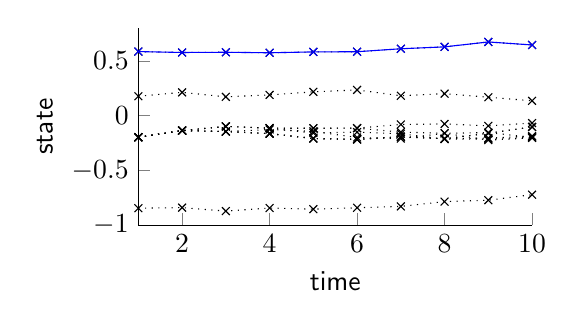
\begin{tikzpicture}

\begin{axis}[%
width=5cm,
height=2.5cm,
scale only axis,
xmin=1,
xmax=10,
xlabel={time},
ymin=-1,
ymax=0.8,
ylabel={state},
axis x line*=bottom,
axis y line*=left
]
\addplot [
color=black,
dotted,
mark=x,
mark options={solid},
forget plot
]
table[row sep=crcr]{
1 -0.845551240007797\\
2 -0.840546836824192\\
3 -0.872080048601409\\
4 -0.84421796719701\\
5 -0.854586924446221\\
6 -0.841810994872285\\
7 -0.829125183937655\\
8 -0.785553434570018\\
9 -0.772567675543346\\
10 -0.721980380882537\\
};
\addplot [
color=black,
dotted,
mark=x,
mark options={solid},
forget plot
]
table[row sep=crcr]{
1 0.178380225849766\\
2 0.213635363813657\\
3 0.172602954084374\\
4 0.190323850620537\\
5 0.218110342445606\\
6 0.235939570950501\\
7 0.182347219287174\\
8 0.201721962940765\\
9 0.169159051260375\\
10 0.136247215714753\\
};
\addplot [
color=black,
dotted,
mark=x,
mark options={solid},
forget plot
]
table[row sep=crcr]{
1 -0.196861446475943\\
2 -0.13598664093345\\
3 -0.144762690908006\\
4 -0.163836263043423\\
5 -0.208286519393592\\
6 -0.21658046659277\\
7 -0.192099174161813\\
8 -0.210809496440697\\
9 -0.160385450854037\\
10 -0.102479059666698\\
};
\addplot [
color=black,
dotted,
mark=x,
mark options={solid},
forget plot
]
table[row sep=crcr]{
1 -0.196861446475943\\
2 -0.13598664093345\\
3 -0.144762690908006\\
4 -0.163836263043423\\
5 -0.208286519393592\\
6 -0.21658046659277\\
7 -0.192099174161813\\
8 -0.210809496440697\\
9 -0.160385450854037\\
10 -0.102479059666698\\
};
\addplot [
color=black,
dotted,
mark=x,
mark options={solid},
forget plot
]
table[row sep=crcr]{
1 -0.196861446475943\\
2 -0.13598664093345\\
3 -0.144762690908006\\
4 -0.163836263043423\\
5 -0.208286519393592\\
6 -0.21658046659277\\
7 -0.192099174161813\\
8 -0.209956267108274\\
9 -0.204663908882357\\
10 -0.185975824479738\\
};
\addplot [
color=black,
dotted,
mark=x,
mark options={solid},
forget plot
]
table[row sep=crcr]{
1 -0.196861446475943\\
2 -0.13598664093345\\
3 -0.144762690908006\\
4 -0.126662292522634\\
5 -0.143404026783185\\
6 -0.199131513361006\\
7 -0.208977769655281\\
8 -0.160638059039865\\
9 -0.222781247847953\\
10 -0.203062717823216\\
};
\addplot [
color=black,
dotted,
mark=x,
mark options={solid},
forget plot
]
table[row sep=crcr]{
1 -0.196861446475943\\
2 -0.13598664093345\\
3 -0.0978611879077818\\
4 -0.113918626941059\\
5 -0.114772220288179\\
6 -0.113550295935696\\
7 -0.149987264343326\\
8 -0.160457205702751\\
9 -0.15412452565722\\
10 -0.198026028555778\\
};
\addplot [
color=black,
dotted,
mark=x,
mark options={solid},
forget plot
]
table[row sep=crcr]{
1 -0.196861446475943\\
2 -0.13598664093345\\
3 -0.0978611879077818\\
4 -0.113918626941059\\
5 -0.114772220288179\\
6 -0.113550295935696\\
7 -0.0801953097596561\\
8 -0.0752702852114935\\
9 -0.0927557198879093\\
10 -0.0671376566914904\\
};
\addplot [
color=black,
dotted,
mark=x,
mark options={solid},
forget plot
]
table[row sep=crcr]{
1 -0.196861446475943\\
2 -0.13598664093345\\
3 -0.0978611879077818\\
4 -0.113918626941059\\
5 -0.158207397501362\\
6 -0.149718292186502\\
7 -0.164943200831398\\
8 -0.214040513386765\\
9 -0.213495448093993\\
10 -0.196080777555403\\
};
\addplot [
color=black,
dotted,
mark=x,
mark options={solid},
forget plot
]
table[row sep=crcr]{
1 0.586442621667069\\
2 0.578187904446798\\
3 0.580168184685444\\
4 0.57551577312066\\
5 0.583282771835473\\
6 0.585189608414548\\
7 0.61215152299557\\
8 0.629592489655878\\
9 0.674435829442097\\
10 0.646877800107992\\
};
\addplot [
color=blue,
solid,
mark=x,
mark options={solid},
forget plot
]
table[row sep=crcr]{
1 0.586442621667069\\
2 0.578187904446798\\
3 0.580168184685444\\
4 0.57551577312066\\
5 0.583282771835473\\
6 0.585189608414548\\
7 0.61215152299557\\
8 0.629592489655878\\
9 0.674435829442097\\
10 0.646877800107992\\
};
\end{axis}
\end{tikzpicture}%
 \caption{A slightly contrived illustration of ineffective backward simulation. Crosses indicate particle filter states, and dotted lines the ancestries. The reference particle is shown with a solid line. A backward simulation sweep does not result in any changes to the reference particle ancestry.}
 \label{fig:bs-fail}
\end{figure}

We can increase the chances of altering the ancestry, and thus further improve mixing of the Markov chain, if the backward simulation algorithm is modified to simultaneously sample a new value for each state along with the corresponding ancestor index. At each time instant we now sample from,
%
\begin{IEEEeqnarray}{rCl}
 \IEEEeqnarraymulticol{3}{l}{ \ed(\an{\ti}\pss{\ai{\ti}}, \ls{\ti}\pss{\ai{\ti}} | \pr, \anset{2:\ti-1}, \lsset{1:\ti-1}, \an{\ti+1:\timax}\pss{\ai{\ti+1:\timax}}, \ls{\ti+1:\timax}\pss{\ai{\ti+1:\timax}}, \aifinal) } \nonumber \\
 \qquad &=& \frac{ \pw{\ti-1}\pss{\an{\ti}\pss{\ai{\ti}}} \td{\ti}(\ls{\ti}\pss{\ai{\ti}}|\ls{\ti-1}\pss{\an{\ti}\pss{\ai{\ti}}}) \od{\ti}(\ob{\ti}|\ls{\ti}\pss{\ai{\ti}}) \td{\ti+1}(\ls{\ti+1}\pss{\ai{\ti+1}}|\ls{\ti}\pss{\ai{\ti}}) }{ \sum_j \pw{\ti-1}\pss{j} \int \td{\ti}(\ls{}|\ls{\ti-1}\pss{j}) \od{\ti}(\ob{\ti}|\ls{}) \td{\ti+1}(\ls{\ti+1}\pss{\ai{\ti+1}}|\ls{}) d\ls{} } \label{eq:rbs-distn}      .
\end{IEEEeqnarray}
%
See appendix~\ref{app:pg-ed-derivations} for a derivation. As before, this is a collapsed Gibbs move. The distribution which we are sampling conceptually is,
%
\begin{IEEEeqnarray}{c}
 \ed(\an{\ti}\pss{\ai{\ti}}, \ls{\ti}\pss{\ai{\ti}}, \anset{\ti:\timax}\pss{\notai{\ti:\timax}}, \lsset{\ti:\timax}\pss{\notai{\ti:\timax}} | \pr, \anset{2:\ti-1}, \lsset{1:\ti-1}, \an{\ti+1:\timax}\pss{\ai{\ti+1:\timax}}, \ls{\ti+1:\timax}\pss{\ai{\ti:\timax}}, \aifinal) \nonumber      .
\end{IEEEeqnarray}
%
However, the non-reference future values need not actually be generated.

% It is straightforward to see that this modified from of PG-BS will mix faster than the standard version. Expanding as,
% %
% \begin{IEEEeqnarray}{rCl}
%  \IEEEeqnarraymulticol{3}{l}{ \ed(\an{\ti}\pss{\ai{\ti}}, \ls{\ti}\pss{\ai{\ti}} | \pr, \anset{2:\ti-1}, \lsset{1:\ti-1}, \an{\ti+1:\timax}\pss{\ai{\ti+1:\timax}}, \ls{\ti+1:\timax}\pss{\ai{\ti+1:\timax}}, \aifinal) } \nonumber \\
%  \qquad &=&  \ed(\an{\ti}\pss{\ai{\ti}} | \pr, \anset{2:\ti-1}, \lsset{1:\ti-1}, \an{\ti+1:\timax}\pss{\ai{\ti+1:\timax}}, \ls{\ti:\timax}\pss{\ai{\ti:\timax}}, \aifinal) \nonumber \\
%  & & \qquad \times \ed(\ls{\ti}\pss{\ai{\ti}} | \pr, \anset{2:\ti-1}, \lsset{1:\ti-1}, \an{\ti+1:\timax}\pss{\ai{\ti+1:\timax}}, \ls{\ti+1:\timax}\pss{\ai{\ti+1:\timax}}, \aifinal) \nonumber      ,
% \end{IEEEeqnarray}
% %
% the new operation is clearly equivalent to an ordinary ancestor sampling stage preceded by an additional state-sampling stage. Additional sampling in each iteration can only improve the mixing of the Markov chain. {\meta Is that true? Citation?} However, this improvement may not be outweighed by the increased computation per iteration needed to sample the state. This trade-off will be dependent on the properties of the particular model in question.
%
% NOT TRUE, BECAUSE WE NO LONGER SAMPLE ANCESTOR DIRECTLY ANY MORE

In standard backward simulation, the conditional for each ancestor index is a categorical distribution \eqref{eq:bs-distn}, which can be sampled directly by evaluating the weight associated with each possible value, or by rejection sampling \citep{Doucet2009,Taghavi2013}. It is also possible to use a Metropolis-Hastings kernel targeting this distribution \citep{Bunch2013,Bunch2014}.

In contrast, the joint conditional for state-ancestor pairs is a mixed continuous-discrete distribution \eqref{eq:rbs-distn}. Since it will not in general be possible to sample from this distribution directly, we consider two possible Markov kernels which can be used instead. To clarify the following explanations, we write the one-step target distribution in a simplified form, omitting superfluous indexes and conditioning,
%
\begin{IEEEeqnarray}{rCl}
\ed(\an{\ti},\ls{\ti} | \lsset{\ti-1}) & = & \frac{ \pw{\ti-1}\pss{\an{\ti}} \utf{\ti}(\ls{\ti}|\ls{\ti-1}\pss{\an{\ti}}) }{ \sum_j \pw{\ti-1}\pss{j} \int \utf{\ti}(\ls{}|\ls{\ti-1}\pss{j}) d\ls{} } \label{eq:simplified-rbs-distn}      .
\end{IEEEeqnarray}

\subsubsection{Metropolis-Hastings}
We can of course target \eqref{eq:simplified-rbs-distn} using Metropolis-Hastings. From current values $\an{\ti}^*$ and $\ls{\ti}^*$, we can propose new values $\an{\ti}'$ and $\ls{\ti}'$ by drawing from,
%
\begin{IEEEeqnarray}{rCl}
 \frac{ \ppw{\ti-1}\pss{\an{\ti}} }{ \sum_j \ppw{\ti-1}\pss{j} } \pd{\ti}(\ls{\ti} | \ls{\ti-1}\pss{\an{\ti}}, \ls{\ti}^*) \label{eq:rbs-mh-ppsl}       ,
\end{IEEEeqnarray}
%
in which $\{\ppw{\ti}\pss{i} : i = 1,\dots,\nump\}$ are a set of proposal weights for the ancestor index and $\pd{\ti}$ is a new proposal density. The resulting acceptance probability is then,
%
\begin{IEEEeqnarray}{rCl}
 \mhap(\an{\ti}^*,\ls{\ti}^* \to \an{\ti}',\ls{\ti}') & = & \min\left\{ 1, \frac{ \pw{\ti-1}\pss{\an{\ti}'} \utf{\ti}(\ls{\ti}'|\ls{\ti-1}\pss{\an{\ti}'}) }{ \ppw{\ti-1}\pss{\an{\ti}'} \pd{\ti}(\ls{\ti}' | \ls{\ti-1}\pss{\an{\ti}'}, \ls{\ti}^*) } \frac{ \ppw{\ti-1}\pss{\an{\ti}^*} \pd{\ti}(\ls{\ti}^* | \ls{\ti-1}\pss{\an{\ti}^*}, \ls{\ti}') }{ \pw{\ti-1}\pss{\an{\ti}^*} \utf{\ti}(\ls{\ti}^*|\ls{\ti-1}\pss{\an{\ti}^*}) } \right\}
\end{IEEEeqnarray}
%
This is the scheme suggested in \citep{Bunch2013,Bunch2014}.


\subsubsection{Conditional Importance Sampling}
The marginal conditional distribution for the ancestor indexes is,
%
\begin{IEEEeqnarray}{rCl}
\ed(\an{\ti} | \lsset{\ti-1}) = \int \ed(\ls{}, \an{\ti} | \lsset{\ti-1}) d\ls{} & = & \frac{ \pw{\ti-1}\pss{\an{\ti}} \int \utf{\ti}(\ls{}|\ls{\ti-1}\pss{\an{\ti}})d\ls{} }{ \sum_j \pw{\ti-1}\pss{j} \int \utf{\ti}(\ls{}|\ls{\ti-1}\pss{j}) d\ls{} } \nonumber      .
\end{IEEEeqnarray}
%
If this distribution is dominated by a small number of possible values with high probability, then a Metropolis-Hastings kernel will be inefficient. It may take a large number of steps before one of these likely ancestors is proposed. In such circumstances it may be advantageous to the following method based \emph{conditional importance sampling} (CIS) instead.

CIS uses the same principle as the conditional particle filter, but applied to a single time step. Suppose we have the current values $\an{\ti}^*$ and $\ls{\ti}^*$, then a Markov kernel may be constructed with \eqref{eq:simplified-rbs-distn} as its invariant distribution by following algorithm~\ref{alg:cis}.

\begin{algorithm}[!h]
\begin{spacing}{1.5}
\begin{algorithmic}[1]
 \REQUIRE Preceding particle states $\lsset{\ti-1}$, current values $\an{\ti}^*$ and $\ls{\ti}^*$.
 \STATE Sample an index uniformly $\cisi^*\in\{1,\dots,\nump\}$.
 \STATE Set $\an{\ti}\pss{\cisi^*} = \an{\ti}^*$. Set $\ls{\ti}\pss{\cisi^*} = \ls{\ti}^*$.
 \FORALL{$i \in \{1,\dots,\nump\}\setminus\cisi^*$}
  \STATE Sample $\an{\ti}\pss{i} \sim \frac{\ppw{\ti-1}\pss{\an{\ti}}}{\sum_j \ppw{\ti-1}\pss{j}}$. Sample $\ls{\ti}\pss{i} \sim \spd{\ti}(\ls{\ti}|\ls{\ti-1}\pss{\an{\ti}\pss{i}})$.
 \ENDFOR
 \STATE Sample $\cisi' \sim \frac{\spw{\ti}\pss{\cisi}}{\sum_j \spw{\ti}\pss{j}}$, where $\spw{\ti} = \frac{ \pw{\ti-1}\pss{\an{\ti}\pss{i}} \utf{\ti}(\ls{\ti}\pss{i}|\ls{\ti-1}\pss{\an{\ti}\pss{i}}) }{ \ppw{\ti-1}\pss{\an{\ti}\pss{i}} \spd{\ti}(\ls{\ti}\pss{i}|\ls{\ti-1}\pss{\an{\ti}\pss{i}}) }$.
 \STATE Set $\an{\ti}' = \an{\ti}\pss{\cisi'}$.
 \STATE Set $\ls{\ti}' = \ls{\ti}\pss{\cisi'}$.
 \RETURN New values $\an{\ti}'$ and $\ls{\ti}'$.
\end{algorithmic}
\end{spacing}
\caption{Conditional importance sampling for the joint ancestor-state conditional distributions.}
\label{alg:cis}
\end{algorithm}

To justify that this is a correct Markov kernel, we construct another extended target distribution over these particles, (Note that this set of particles is separate to that of the primary Gibbs sampler.)
%
\begin{IEEEeqnarray}{rCl}
 \cised(\anset{\ti}, \lsset{\ti}, \cisi) & = & \frac{1}{\nump} \ed(\ls{\ti}\pss{\cisi}, \an{\ti}\pss{\cisi} | \lsset{\ti-1}) \times \prod_{i\ne\cisi} \frac{\ppw{\ti}\pss{\an{\ti}\pss{i}}}{\sum_j \ppw{\ti}\pss{j}} \spd{\ti}(\ls{\ti}\pss{i}|\ls{\ti-1}\pss{\an{\ti}\pss{i}}) 
\end{IEEEeqnarray}
%
The first part of algorithm~\ref{alg:cis} by construction corresponds to sampling from the conditional distribution, $\cised(\anset{\ti}\pss{\notcisi}, \lsset{\ti}\pss{\notcisi} | \an{\ti}\pss{\cisi}, \ls{\ti}\pss{\cisi}, \cisi)$, and the final part to sampling from $\cised(\cisi|\anset{\ti}, \lsset{\ti})$. See appendix~\ref{app:cis-ed-derivations} for a proof.

Hence, if the starting values are distributed according to the desired posterior, then the final values must also be, and so the procedure is a Markov kernel with the desired invariant distribution.

\section{Extensions and Variations}

\subsection{Multiple Time Steps}

In extreme cases, even with refreshed backward simulation the update rate of the earliest states may be low. If this occurs, it is may be beneficial to extend the method to sample states at multiple steps, thus giving us yet more leeway to match the sampled future to the possible particle histories. At each time instant we now sample from,
%
\begin{IEEEeqnarray}{rCl}
 \IEEEeqnarraymulticol{3}{l}{ \ed(\an{\ti}\pss{\ai{\ti}}, \ls{\ti:\ti+\wl-1}\pss{\ai{\ti:\ti+\wl-1}} | \pr, \lsset{1:\ti-1}, \anset{2:\ti-1}, \ls{\ti+\wl:\timax}\pss{\ai{\ti+\wl:\timax}}, \an{\ti+1:\timax}\pss{\ai{\ti+1:\timax}}, \aifinal) } \nonumber \\
 \qquad &\propto& \pw{\ti-1}\pss{\an{\ti}\pss{\ai{\ti}}} \td{\ti+\wl}(\ls{\ti+\wl}\pss{\ai{\ti+\wl}}|\ls{\ti+\wl-1}\pss{\ai{\ti+\wl-1}}) \prod_{k=\ti}^{\ti+\wl-1} \td{k}(\ls{k}\pss{\ai{k}}|\ls{k-1}\pss{\an{k}\pss{\ai{k}}}) \od{k}(\ob{k}|\ls{k}\pss{\ai{k}}) \nonumber      .
\end{IEEEeqnarray}

As before, this is a collapsed Gibbs move. The distribution which we are sampling conceptually is,
%
\begin{IEEEeqnarray}{c}
 \ed(\an{\ti}\pss{\ai{\ti}}, \ls{\ti:\ti+\wl-1}\pss{\ai{\ti:\ti+\wl-1}}, \anset{\ti:\timax}\pss{\notai{\ti:\timax}}, \lsset{\ti:\timax}\pss{\notai{\ti:\timax}} | \pr, \lsset{1:\ti-1}, \anset{2:\ti-1}, \ls{\ti+\wl:\timax}\pss{\ai{\ti+\wl:\timax}}, \an{\ti+1:\timax}\pss{\ai{\ti+1:\timax}} \aifinal) \nonumber      .
\end{IEEEeqnarray}
%
However, the non-reference future values need not actually be generated. Implementing such a scheme will require careful design of proposal or importance densities for the joining bridge of state $\ls{\ti:\ti+\wl-1}\pss{\ai{\ti:\ti+\wl-1}}$.


\subsection{Ancestor Sampling}

Rather than conducting the complete forward sweep (i.e. the conditional particle filter) followed by a backward simulation sweep, the steps of the two may be interleaved. This is the basis of particle Gibbs with ancestor sampling (PG-AS) \citep{Lindsten2014}. At time step $\ti$, we would first sample from,
%
\begin{IEEEeqnarray}{rCl}
 \ed(\anset{\ti}\pss{\notai{\ti}}, \lsset{\ti}\pss{\notai{\ti}} | \pr, \anset{1:\ti-1}, \lsset{1:\ti-1}, \an{2:\timax}\pss{\ai{2:\timax}}, \ls{1:\timax}\pss{\ai{1:\timax}}, \aifinal) \nonumber     ,
\end{IEEEeqnarray}
%
and then from,
%
\begin{IEEEeqnarray}{rCl}
 \ed(\an{\ti}\pss{\ai{\ti}}, \ls{\ti}\pss{\ai{\ti}} | \pr, \anset{2:\ti-1}, \lsset{1:\ti-1}, \an{\ti+1:\timax}\pss{\ai{\ti+1:\timax}}, \ls{\ti+1:\timax}\pss{\ai{\ti+1:\timax}}, \aifinal) \nonumber     .
\end{IEEEeqnarray}
%


\section{Simulations}

\subsection{The Model}
Particle Gibbs (PG), Particle Gibbs with Backward Simulation (PG-BS) and Particle Gibbs with Refreshed Backward Simulation (PG-RBS) were tested on a tracking model. The transition model is 3D near constant velocity motion \citep{Li2003}, and the observation model is noisy measurements of bearing, elevation and range. The parameter to be learned is the scale factor on the transition covariance matrix $\sigma^2$, which characterises the target manoeuvrability. Data sets are simulated from the model, each with 100 time steps. An uninformative conjugate prior is used for $\sigma^2$.

\subsection{Algorithm Settings}
The algorithms were each run on $5$ different simulated data sets. Each algorithm was run for 5000 iterations, with a burn in of 1000. PG and PG-BS were run twice, with 100 and 200 particles each. PG-RBS was run with 100 particles. PG-RBS with 100 particles takes roughly the same time as PG-BS with 200 particles.

The particle filter uses a Kalman filter approximation to the optimal importance density,
%
\begin{IEEEeqnarray}{rCl}
 \id{\ti}(\ls{\ti}|\ls{\ti-1}) & \approx & \den(\ls{\ti}|\ls{\ti-1},\ob{\ti}) \nonumber     .
\end{IEEEeqnarray}
%
PG-RBS is implemented with the conditional importance sampling method using a similar Gaussian approximation for the importance density,
%
\begin{IEEEeqnarray}{rCl}
 \spd{\ti}(\ls{\ti}|\ls{\ti-1}) & \approx & \den(\ls{\ti}|\ls{\ti-1},\ls{\ti+1},\ob{\ti}) \nonumber     .
\end{IEEEeqnarray}
%
For the proposal weights, we use $\ppw{\ti}\pss{i}=\pw{\ti}\pss{i}$.


\subsection{Results}
PG does not mix well at all. Parameter estimates do not approach the true value, even after 5000 iterations. PG-BS and PG-RBS do converge. Figure~\ref{fig:sample_hist} shows the posterior histograms and figure~\ref{fig:acf} the mean autocorrelation function over the $5$ simulations. The latter indicates faster mixing from PG-RBS with both equal-time and equal-particle equivalents.

\begin{figure}
\centering
\subfloat[PG-BS (N=100)]{ % This file was created by matlab2tikz v0.4.4 running on MATLAB 8.3.
% Copyright (c) 2008--2013, Nico Schlömer <nico.schloemer@gmail.com>
% All rights reserved.
% 
% The latest updates can be retrieved from
%   http://www.mathworks.com/matlabcentral/fileexchange/22022-matlab2tikz
% where you can also make suggestions and rate matlab2tikz.
% 
%
% defining custom colors
\definecolor{mycolor1}{rgb}{0,0,0.5625}%
%
\begin{tikzpicture}

\begin{axis}[%
width=4.5cm,
height=4.5cm,
area legend,
scale only axis,
xmin=0.5,
xmax=2,
xlabel={$\sigma^2$},
ymin=0,
ymax=500,
axis x line*=bottom,
axis y line*=left
]
\addplot[ybar,bar width=0.170085103120214cm,draw=black,fill=mycolor1] plot coordinates{(0.710612054054637,26)
(0.761637584990702,67)
(0.812663115926766,118)
(0.86368864686283,196)
(0.914714177798895,271)
(0.965739708734959,390)
(1.01676523967102,394)
(1.06779077060709,410)
(1.11881630154315,390)
(1.16984183247922,351)
(1.22086736341528,308)
(1.27189289435134,274)
(1.32291842528741,195)
(1.37394395622347,145)
(1.42496948715954,101)
(1.4759950180956,81)
(1.52702054903167,56)
(1.57804607996773,47)
(1.62907161090379,31)
(1.68009714183986,34)
(1.73112267277592,26)
(1.78214820371199,22)
(1.83317373464805,20)
(1.88419926558412,11)
(1.93522479652018,7)
(1.98625032745624,8)
(2.03727585839231,7)
(2.08830138932837,8)
(2.13932692026444,4)
(2.1903524512005,2)};

\addplot [
color=black,
solid,
forget plot
]
table[row sep=crcr]{
0.5 0\\
2 0\\
};
\addplot [
color=black,
dotted,
forget plot
]
table[row sep=crcr]{
1 0\\
1 500\\
};
\end{axis}
\end{tikzpicture}% }
\subfloat[PG-BS (N=200)]{ % This file was created by matlab2tikz v0.4.4 running on MATLAB 8.3.
% Copyright (c) 2008--2013, Nico Schlömer <nico.schloemer@gmail.com>
% All rights reserved.
% 
% The latest updates can be retrieved from
%   http://www.mathworks.com/matlabcentral/fileexchange/22022-matlab2tikz
% where you can also make suggestions and rate matlab2tikz.
% 
%
% defining custom colors
\definecolor{mycolor1}{rgb}{0,0,0.5625}%
%
\begin{tikzpicture}

\begin{axis}[%
width=4.5cm,
height=4.5cm,
area legend,
scale only axis,
xmin=0.5,
xmax=2,
xlabel={$\sigma^2$},
ymin=0,
ymax=500,
axis x line*=bottom,
axis y line*=left
]
\addplot[ybar,bar width=0.178998656193082cm,draw=black,fill=mycolor1] plot coordinates{(0.694917780309864,21)
(0.748617377167789,37)
(0.802316974025714,94)
(0.856016570883639,222)
(0.909716167741564,320)
(0.96341576459949,423)
(1.01711536145741,350)
(1.07081495831534,373)
(1.12451455517326,380)
(1.17821415203119,311)
(1.23191374888912,318)
(1.28561334574704,288)
(1.33931294260497,235)
(1.39301253946289,186)
(1.44671213632082,129)
(1.50041173317874,88)
(1.55411133003667,65)
(1.60781092689459,33)
(1.66151052375252,23)
(1.71521012061044,19)
(1.76890971746837,13)
(1.82260931432629,16)
(1.87630891118422,12)
(1.93000850804214,17)
(1.98370810490007,14)
(2.03740770175799,5)
(2.09110729861592,4)
(2.14480689547384,3)
(2.19850649233177,0)
(2.25220608918969,1)};

\addplot [
color=black,
solid,
forget plot
]
table[row sep=crcr]{
0.5 0\\
2 0\\
};
\addplot [
color=black,
dotted,
forget plot
]
table[row sep=crcr]{
1 0\\
1 500\\
};
\end{axis}
\end{tikzpicture}% } \\
\subfloat[PG-RBS (N=100)]{ % This file was created by matlab2tikz v0.4.4 running on MATLAB 8.3.
% Copyright (c) 2008--2013, Nico Schlömer <nico.schloemer@gmail.com>
% All rights reserved.
% 
% The latest updates can be retrieved from
%   http://www.mathworks.com/matlabcentral/fileexchange/22022-matlab2tikz
% where you can also make suggestions and rate matlab2tikz.
% 
%
% defining custom colors
\definecolor{mycolor1}{rgb}{0,0,0.5625}%
%
\begin{tikzpicture}

\begin{axis}[%
width=4.5cm,
height=4.5cm,
area legend,
scale only axis,
xmin=0.5,
xmax=2,
xlabel={$\sigma^2$},
ymin=0,
ymax=500,
axis x line*=bottom,
axis y line*=left
]
\addplot[ybar,bar width=0.135812392440373cm,draw=black,fill=mycolor1] plot coordinates{(0.607294061023861,4)
(0.648037778755973,4)
(0.688781496488085,29)
(0.729525214220197,36)
(0.77026893195231,105)
(0.811012649684422,155)
(0.851756367416534,249)
(0.892500085148646,291)
(0.933243802880758,337)
(0.973987520612871,369)
(1.01473123834498,329)
(1.0554749560771,355)
(1.09621867380921,314)
(1.13696239154132,290)
(1.17770610927343,254)
(1.21844982700554,185)
(1.25919354473766,172)
(1.29993726246977,128)
(1.34068098020188,120)
(1.38142469793399,100)
(1.4221684156661,51)
(1.46291213339822,42)
(1.50365585113033,25)
(1.54439956886244,20)
(1.58514328659455,13)
(1.62588700432667,9)
(1.66663072205878,7)
(1.70737443979089,3)
(1.748118157523,3)
(1.78886187525511,1)};

\addplot [
color=black,
solid,
forget plot
]
table[row sep=crcr]{
0.5 0\\
2 0\\
};
\addplot [
color=black,
dotted,
forget plot
]
table[row sep=crcr]{
1 0\\
1 500\\
};
\end{axis}
\end{tikzpicture}% }
\caption{Posterior sample histograms.}
\label{fig:sample_hist}
\end{figure}

\begin{figure}
\centering
% This file was created by matlab2tikz v0.4.4 running on MATLAB 8.3.
% Copyright (c) 2008--2013, Nico Schlömer <nico.schloemer@gmail.com>
% All rights reserved.
% 
% The latest updates can be retrieved from
%   http://www.mathworks.com/matlabcentral/fileexchange/22022-matlab2tikz
% where you can also make suggestions and rate matlab2tikz.
% 
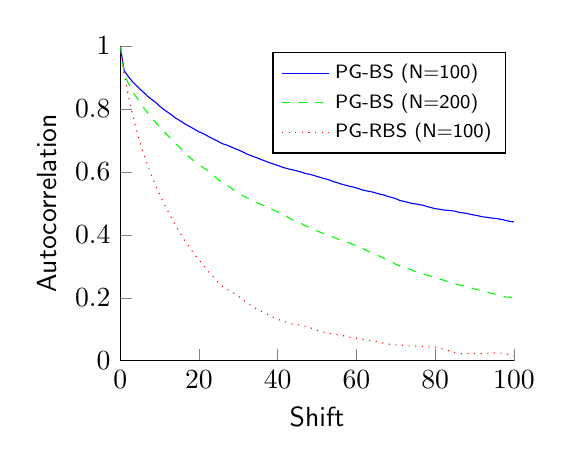
\begin{tikzpicture}

\begin{axis}[%
width=5cm,
height=4cm,
scale only axis,
xmin=0,
xmax=100,
xlabel={Shift},
ymin=0,
ymax=1,
ylabel={Autocorrelation},
axis x line*=bottom,
axis y line*=left,
legend style={draw=black,fill=white,legend cell align=left,font=\scriptsize}
]
\addplot [
color=blue,
solid
]
table[row sep=crcr]{
0 0.999903588398655\\
1 0.920486758741033\\
2 0.903335600089798\\
3 0.887932912664518\\
4 0.875071561743713\\
5 0.862746477492585\\
6 0.851314107455174\\
7 0.839539717987804\\
8 0.829617302754404\\
9 0.819980096411471\\
10 0.80851358299916\\
11 0.798425692380472\\
12 0.789661712034424\\
13 0.781040752052782\\
14 0.770955684745448\\
15 0.763721647120573\\
16 0.755612497589696\\
17 0.747979350271797\\
18 0.74125998446863\\
19 0.734015903212486\\
20 0.726885609263636\\
21 0.721774805650458\\
22 0.714834974081635\\
23 0.70817942947304\\
24 0.701898147848601\\
25 0.695616649427075\\
26 0.688974608321642\\
27 0.6851970987231\\
28 0.680062512922832\\
29 0.6742958539347\\
30 0.669354507938002\\
31 0.663801465676009\\
32 0.657324012584225\\
33 0.652239054507617\\
34 0.647495753789502\\
35 0.642939438890071\\
36 0.63803813715115\\
37 0.633199398445475\\
38 0.628545342669218\\
39 0.624336512986373\\
40 0.620238414860391\\
41 0.615311934916251\\
42 0.611695957499656\\
43 0.608310727704075\\
44 0.60550665634806\\
45 0.602463687990571\\
46 0.599238899231897\\
47 0.594598732631037\\
48 0.592495930677031\\
49 0.589200399894096\\
50 0.585110833142028\\
51 0.581402529342026\\
52 0.577920187311273\\
53 0.574500259063287\\
54 0.569415472560249\\
55 0.565955441292513\\
56 0.561673158412858\\
57 0.558083952812055\\
58 0.554806799771933\\
59 0.55219885880144\\
60 0.54844815006866\\
61 0.544501785509853\\
62 0.540985283756493\\
63 0.538066109300578\\
64 0.536001441562287\\
65 0.532198410435559\\
66 0.528996414229476\\
67 0.526309604928353\\
68 0.521589368070406\\
69 0.518658366353822\\
70 0.514465745513353\\
71 0.508946063401548\\
72 0.506226975519337\\
73 0.503134011096087\\
74 0.499868691306728\\
75 0.498066451993802\\
76 0.495571368463879\\
77 0.49355915035869\\
78 0.489197877917402\\
79 0.486131482756531\\
80 0.482969539462418\\
81 0.481372073527897\\
82 0.479024702393476\\
83 0.477740704816924\\
84 0.476640239654847\\
85 0.475103985782292\\
86 0.471327335736112\\
87 0.46968554058109\\
88 0.467853043993988\\
89 0.464760815570657\\
90 0.462341589505022\\
91 0.460176468560824\\
92 0.457070342540286\\
93 0.455870346197615\\
94 0.453600076942254\\
95 0.452398031197086\\
96 0.450827856118165\\
97 0.448215475094587\\
98 0.445449836835981\\
99 0.442224738235369\\
100 0.441071594680408\\
};
\addlegendentry{PG-BS (N=100)};

\addplot [
color=green,
dashed
]
table[row sep=crcr]{
0 0.999891622509946\\
1 0.9131246158294\\
2 0.882590227019065\\
3 0.8582602335872\\
4 0.83864457797386\\
5 0.820362545887663\\
6 0.802387098269211\\
7 0.786505235036271\\
8 0.770814721666268\\
9 0.757092639968614\\
10 0.742342348503673\\
11 0.728497879036039\\
12 0.716143443561847\\
13 0.703853923211808\\
14 0.691396752686264\\
15 0.677772859360532\\
16 0.666288650358538\\
17 0.653209238540924\\
18 0.641498206692758\\
19 0.632365913374451\\
20 0.622792424946645\\
21 0.614121802860441\\
22 0.60537280475484\\
23 0.594313485223001\\
24 0.583971860831792\\
25 0.573835170993497\\
26 0.566436191669736\\
27 0.558552263209654\\
28 0.549839340354118\\
29 0.540130464552977\\
30 0.532755589171176\\
31 0.524876622654475\\
32 0.51855139173525\\
33 0.511278961624043\\
34 0.506446429199656\\
35 0.499705126430569\\
36 0.494845992349021\\
37 0.488700271131707\\
38 0.484018516707596\\
39 0.478072697855192\\
40 0.472090833324776\\
41 0.466513223118886\\
42 0.460223428261561\\
43 0.452526218331281\\
44 0.445328368759231\\
45 0.440265398222439\\
46 0.435392297235818\\
47 0.428947618670154\\
48 0.423183579560225\\
49 0.417462989012893\\
50 0.411995013201967\\
51 0.407205932684084\\
52 0.402207830935458\\
53 0.397922306870715\\
54 0.393058219680795\\
55 0.387814257947974\\
56 0.383033023373619\\
57 0.378414999882359\\
58 0.374851280357911\\
59 0.369324121495941\\
60 0.364867272184509\\
61 0.359489327007041\\
62 0.353595077317804\\
63 0.347355069614687\\
64 0.341719696683109\\
65 0.336888527985878\\
66 0.331428006813312\\
67 0.324761659342965\\
68 0.319013074482997\\
69 0.313271440290862\\
70 0.306303817457784\\
71 0.301138009026498\\
72 0.297389379001777\\
73 0.29347833550842\\
74 0.288296196445506\\
75 0.282584345673744\\
76 0.279371813047442\\
77 0.275157239074421\\
78 0.272128280457854\\
79 0.267272972722048\\
80 0.264261166815676\\
81 0.260413975258518\\
82 0.256436206347447\\
83 0.251588116325574\\
84 0.248496252124085\\
85 0.243938512892472\\
86 0.241065536660925\\
87 0.238299602509428\\
88 0.235290538187007\\
89 0.232054998039984\\
90 0.227924449045455\\
91 0.224588471187677\\
92 0.221257774791747\\
93 0.217308396373018\\
94 0.215075613077136\\
95 0.211706605033252\\
96 0.207989158206567\\
97 0.206486957352932\\
98 0.202275599725738\\
99 0.201825138277393\\
100 0.199200058201334\\
};
\addlegendentry{PG-BS (N=200)};

\addplot [
color=red,
dotted
]
table[row sep=crcr]{
0 0.999836856429826\\
1 0.910398688836733\\
2 0.844782150614985\\
3 0.787620042324497\\
4 0.737853651209422\\
5 0.693994838677503\\
6 0.654315850392674\\
7 0.618568217625445\\
8 0.586195338684792\\
9 0.556818731672658\\
10 0.528109497284171\\
11 0.502829814719507\\
12 0.477350566982722\\
13 0.453688901611592\\
14 0.430564363314501\\
15 0.40897930305615\\
16 0.389484210518673\\
17 0.370964783991475\\
18 0.353018700995438\\
19 0.33540299548346\\
20 0.319933653980552\\
21 0.305356253628572\\
22 0.289179203425347\\
23 0.274406042861078\\
24 0.261304135708604\\
25 0.247755998137365\\
26 0.236061687396796\\
27 0.227463781647957\\
28 0.220244136793719\\
29 0.213287617224539\\
30 0.20490129570517\\
31 0.195880371291582\\
32 0.186137927637386\\
33 0.177132772427266\\
34 0.169414673416553\\
35 0.161318486645558\\
36 0.155992486114113\\
37 0.14976022437866\\
38 0.144525499746458\\
39 0.136632852447348\\
40 0.131445190441772\\
41 0.127907247448965\\
42 0.123132985717143\\
43 0.11952692899989\\
44 0.115364350672671\\
45 0.114805238457567\\
46 0.112324292775659\\
47 0.109479786360627\\
48 0.105858668864598\\
49 0.101598658448661\\
50 0.0969952588664834\\
51 0.0932471617431775\\
52 0.0900665289146602\\
53 0.0871118085891429\\
54 0.0850219392513513\\
55 0.0828455892510456\\
56 0.0814442204557225\\
57 0.0785079304935199\\
58 0.0747592673039743\\
59 0.0735481626352929\\
60 0.0716276326337509\\
61 0.069873210243891\\
62 0.0667399310572844\\
63 0.0649374977859129\\
64 0.0629298967091192\\
65 0.0611635809746716\\
66 0.058076033541349\\
67 0.0556469569111609\\
68 0.0533158867783404\\
69 0.0517332091355979\\
70 0.050111071873803\\
71 0.0498392679342351\\
72 0.048673904316628\\
73 0.0476411846370012\\
74 0.0471502717819124\\
75 0.046694203985966\\
76 0.0459429594082649\\
77 0.0450003431629298\\
78 0.0443270395112047\\
79 0.0443381644899684\\
80 0.0432467756119263\\
81 0.0414659584998818\\
82 0.0372622166510958\\
83 0.0334647377790083\\
84 0.0295848968740434\\
85 0.0259132126267024\\
86 0.0232463565628023\\
87 0.0222163617765922\\
88 0.0223982565101699\\
89 0.0228233732461777\\
90 0.0225172441669789\\
91 0.0228275365879988\\
92 0.0231265577263647\\
93 0.0230560657873127\\
94 0.0236575228549241\\
95 0.0252025267224022\\
96 0.023964658362867\\
97 0.024175673155557\\
98 0.0224850074230927\\
99 0.0186754976327629\\
100 0.0161258088535605\\
};
\addlegendentry{PG-RBS (N=100)};

\end{axis}
\end{tikzpicture}%
\caption{Mean autocorrelation function for PG-BS and PG-RBS.}
\label{fig:acf}
\end{figure}


\section{Summary and Conclusions}

We have introduced a simple but effective modification to particle Gibbs which can significantly improve the mixing of the Markov chains. Rather than running a standard backward simulation sweep after each iteration of the conditional particle filter, we use refreshed backward simulation, in which new values of the states of the reference trajectory are sampled along with their corresponding ancestor indexes. Direct sampling of the appropriate conditional distributions is not generally possible, however suitable Markov kernels are available instead. As well as basic Metropolis-Hastings, we have presented a kernel based on conditional importance sampling. Simulations on a simple tracking model have demonstrated substantial improvements in Markov chain autocorrelation. 


\clearpage

\appendix

\section{Particle Gibbs Extended Target Conditionals} \label{app:pg-ed-derivations}

This appendix contains derivations of the conditionals of the extended target distribution required to implement particle Gibbs in its various forms.

\subsection{Extended Target Distribution}

The particle MCMC extended target distribution is,
%
\begin{IEEEeqnarray}{rCl}
 \ed(\pr, \anset{2:\timax}, \lsset{1:\timax}, \aifinal) & = & \frac{1}{\nump^\timax} \den(\pr, \ls{1:\timax}\pss{\ai{1:\timax}}|\ob{1:\timax}) \nonumber \\
  & & \qquad  \times \prod_{i\ne\ai{1}} \id{1}(\ls{1}\pss{i}) \prod_{\ti=2}^{\timax} \left[ \prod_{i\ne\ai{\ti}} \frac{ \pw{\ti-1}\pss{\an{\ti}\pss{i}} }{ \sum_j \pw{\ti-1}\pss{j} } \id{\ti}(\ls{\ti}\pss{i}|\ls{\ti-1}\pss{\an{\ti}\pss{i}}) \right] \label{app-eq:extended_dist_v1}     .
\end{IEEEeqnarray}
%
By design, this has,
%
\begin{IEEEeqnarray}{rCl}
 \ed(\pr, \an{2:\timax}\pss{\ai{\ti}}, \ls{1:\timax}\pss{\ai{\ti}}, \aifinal) & = & \frac{1}{\nump^\timax} \den(\pr, \ls{1:\timax}\pss{\ai{1:\timax}}|\ob{1:\timax}) \nonumber      ,
\end{IEEEeqnarray}
%
and,
%
\begin{IEEEeqnarray}{rCl}
 \IEEEeqnarraymulticol{3}{l}{ \ed(\lsset{1:\timax}\pss{\notai{1:\timax}}, \anset{2:\timax}\pss{\notai{2:\timax}} | \pr, \ls{1:\timax}\pss{\ai{1:\timax}}, \an{2:\timax}\pss{\ai{2:\timax}}, \aifinal) } \nonumber \\
 \qquad & = & \prod_{i\ne\ai{1}} \id{1}(\ls{1}\pss{i}) \prod_{\ti=1}^{\timax} \left[ \prod_{i\ne\ai{\ti}} \frac{ \pw{\ti-1}\pss{\an{\ti}\pss{i}} }{ \sum_j \pw{\ti-1}\pss{j} } \id{\ti}(\ls{\ti}\pss{i}|\ls{\ti-1}\pss{\an{\ti}\pss{i}}) \right] \nonumber     .
\end{IEEEeqnarray}
%
Sampling this latter distribution corresponds to the conditional particle filter routine.

The final stage of particle Gibbs is to sample an index $\aifinal$ which indicates one of the trajectories to be the reference. To derive the necessary conditional, begin by expanding the posterior term using Bayes rule,
%
\begin{IEEEeqnarray}{rCl}
 \den(\pr, \ls{1:\timax}\pss{\ai{1:\timax}}|\ob{1:\timax}) & = & \frac{1}{\den(\ob{1:\timax})} \prod_{\ti=1}^{\timax} \td{\ti}(\ls{\ti}\pss{\ai{\ti}}|\ls{\ti-1}\pss{\ai{\ti-1}}) \od{\ti}(\ob{\ti}|\ls{\ti}\pss{\ai{\ti}})  \nonumber      .
\end{IEEEeqnarray}
%
Then by repeatedly using the definition of the particle weights, and the fact that $\ai{\ti}=\an{\ti+1}\pss{\ai{\ti+1}}$,
%
\begin{IEEEeqnarray}{rCl}
 \IEEEeqnarraymulticol{3}{l}{ \prod_{\ti=1}^{\timax} \td{\ti}(\ls{\ti}\pss{\ai{\ti}}|\ls{\ti-1}\pss{\ai{\ti-1}}) \od{\ti}(\ob{\ti}|\ls{\ti}\pss{\ai{\ti}}) } \nonumber \\
 \qquad & = & \pw{\timax}\pss{\aifinal} \id{1}(\ls{1}\pss{\ai{1}}) \prod_{\ti=2}^{\timax} \pw{\ti-1}\pss{\an{\ti}\pss{\ai{\ti}}} \id{\ti}(\ls{\ti}\pss{\ai{\ti}}|\ls{\ti-1}\pss{\an{\ti}\pss{\ai{\ti}}}) \label{app-eq:recursive-weight-def}     .
\end{IEEEeqnarray}
%
Using these we rearrange the extended target as,
%
\begin{IEEEeqnarray}{rCl}
 \ed(\pr, \anset{2:\timax}, \lsset{1:\timax}, \aifinal) & = & \frac{\prod_{\ti=1}^{\timax}\left[\sum_j \pw{\ti}\pss{j}\right]}{\nump^\timax \: \den(\ob{1:\timax})} \times \frac{ \pw{\timax}\pss{\aifinal} }{\sum_j \pw{\timax}\pss{j} } \nonumber \\
  & & \qquad  \times \prod_{i} \id{1}(\ls{1}\pss{i}) \prod_{\ti=2}^{\timax} \left[ \prod_{i} \frac{ \pw{\ti-1}\pss{\an{\ti}\pss{i}} }{ \sum_j \pw{\ti-1}\pss{j} } \id{\ti}(\ls{\ti}\pss{i}|\ls{\ti-1}\pss{\an{\ti}\pss{i}}) \right] \label{app-eq:extended_dist_v2}     .
\end{IEEEeqnarray}
%
Hence, the required conditional is clearly,
%
\begin{IEEEeqnarray}{rCl}
 \ed(\aifinal|\pr, \lsset{1:\timax}, \anset{2:\timax}) &=& \frac{\pw{\timax}\pss{\aifinal}}{\sum_j \pw{\timax}\pss{j}} \nonumber      .
\end{IEEEeqnarray}

\subsection{Backward Simulation}

Backward simulation corresponds to a sweep backwards through time sampling at each time instant from,
%
\begin{IEEEeqnarray}{rCl}
 \IEEEeqnarraymulticol{3}{l}{ \ed(\an{\ti}\pss{\ai{\ti}} | \pr, \anset{1:\ti-1}, \lsset{1:\ti-1}, \an{\ti+1:\timax}\pss{\ai{\ti+1:\timax}}, \ls{\ti:\timax}\pss{\ai{\ti:\timax}}, \aifinal) } \nonumber \\
 \qquad & = & \frac{ \ed(\pr, \anset{1:\ti-1}, \lsset{1:\ti-1}, \an{\ti:\timax}\pss{\ai{\ti:\timax}}, \ls{\ti:\timax}\pss{\ai{\ti:\timax}}, \aifinal) }{ \ed(\pr, \anset{1:\ti-1}, \lsset{1:\ti-1}, \an{\ti+1:\timax}\pss{\ai{\ti+1:\timax}}, \ls{\ti:\timax}\pss{\ai{\ti:\timax}}, \aifinal) } \nonumber     .
\end{IEEEeqnarray}
%
It is straightforward to marginalise the non-reference trajectory future states and ancestor indexes from the extended target distribution. Simply proceed backwards in time, alternately integrating out the last state and then summing over the ancestor values. See \citep{Olsson2011}. This leaves us with,
%
\begin{IEEEeqnarray}{rCl}
 \IEEEeqnarraymulticol{3}{l}{ \ed(\pr, \anset{1:\ti-1}, \lsset{1:\ti-1}, \an{\ti:\timax}\pss{\ai{\ti:\timax}}, \ls{\ti:\timax}\pss{\ai{\ti:\timax}}, \aifinal) } \nonumber \\
 \qquad & = & \frac{1}{\nump^\timax} \den(\pr, \ls{1:\timax}\pss{\ai{1:\timax}}|\ob{1:\timax}) \prod_{i\ne\ai{1}} \id{1}(\ls{1}\pss{i}) \prod_{\ti=2}^{\ti-1} \left[ \prod_{i\ne\ai{\ti}} \frac{ \pw{\ti-1}\pss{\an{\ti}\pss{i}} }{ \sum_j \pw{\ti-1}\pss{j} } \id{\ti}(\ls{\ti}\pss{i}|\ls{\ti-1}\pss{\an{\ti}\pss{i}}) \right] \nonumber     .
\end{IEEEeqnarray}
%
Using Bayes rule, write the posterior term as,
%
\begin{IEEEeqnarray}{rCl}
 \den(\pr, \ls{1:\timax}\pss{\ai{1:\timax}}|\ob{1:\timax}) & = & \frac{1}{\den(\ob{1:\timax})} \den(\ob{\ti:\timax},\ls{\ti+1:\timax}\pss{\ai{\ti+1:\timax}}|\ls{\ti}\pss{\ai{\ti}}) \td{\ti}(\ls{\ti}\pss{\ai{\ti}}|\ls{\ti-1}\pss{\ai{\ti-1}}) \nonumber \\
 & & \qquad \times \prod_{k=1}^{\ti-1} \td{k}(\ls{k}\pss{\ai{k}}|\ls{k-1}\pss{\ai{k-1}}) \od{k}(\ob{k}|\ls{k}\pss{\ai{k}})  \nonumber      ,
\end{IEEEeqnarray}
%
and then applying \eqref{app-eq:recursive-weight-def}, we find,
%
\begin{IEEEeqnarray}{rCl}
  \IEEEeqnarraymulticol{3}{l}{ \ed(\pr, \anset{1:\ti-1}, \lsset{1:\ti-1}, \an{\ti:\timax}\pss{\ai{\ti:\timax}}, \ls{\ti:\timax}\pss{\ai{\ti:\timax}}, \aifinal) } \nonumber \\
 \qquad & = & \frac{ \den(\ob{\ti:\timax},\ls{\ti+1:\timax}\pss{\ai{\ti+1:\timax}}|\ls{\ti}\pss{\ai{\ti}}) }{ \nump^\timax \den(\ob{1:\timax}) } \prod_{k=2}^{\ti-1} \left[\sum_j \pw{k-1}\pss{j}\right] \nonumber \\ 
  & & \qquad \times \prod_{i} \id{1}(\ls{1}\pss{i}) \prod_{\ti=2}^{\ti-1} \left[ \prod_{i} \frac{ \pw{\ti-1}\pss{\an{\ti}\pss{i}} }{ \sum_j \pw{\ti-1}\pss{j} } \id{\ti}(\ls{\ti}\pss{i}|\ls{\ti-1}\pss{\an{\ti}\pss{i}}) \right] \nonumber \\
  & & \qquad \times \pw{\ti-1}\pss{\an{\ti}\pss{\ai{\ti}}} \td{\ti}(\ls{\ti}\pss{\ai{\ti}}|\ls{\ti-1}\pss{\an{\ti}\pss{\ai{\ti}}}) \nonumber     ,
\end{IEEEeqnarray}
%
% And hence, marginalising over $\an{\ti}\pss{\ai{\ti}}$,
% %
% \begin{IEEEeqnarray}{rCl}
%   \IEEEeqnarraymulticol{3}{l}{ \ed(\pr, \anset{1:\ti-1}, \lsset{1:\ti-1}, \an{\ti:\timax}\pss{\ai{\ti:\timax}}, \ls{\ti:\timax}\pss{\ai{\ti:\timax}}, \aifinal) } \nonumber \\
%  \qquad & = & \frac{ \den(\ob{\ti:\timax},\ls{\ti+1:\timax}\pss{\ai{\ti+1:\timax}}|\ls{\ti}\pss{\ai{\ti}}) }{ \nump^\timax \den(\ob{1:\timax}) } \prod_{k=2}^{\ti-1} \left[\sum_j \pw{k-1}\pss{j}\right] \nonumber \\ 
%   & & \qquad \times \prod_{i} \id{1}(\ls{1}\pss{i}) \prod_{\ti=2}^{\ti-1} \left[ \prod_{i} \frac{ \pw{\ti-1}\pss{\an{\ti}\pss{i}} }{ \sum_j \pw{\ti-1}\pss{j} } \id{\ti}(\ls{\ti}\pss{i}|\ls{\ti-1}\pss{\an{\ti}\pss{i}}) \right] \nonumber \\
%   & & \qquad \times \sum_j \pw{\ti-1}\pss{j} \td{\ti}(\ls{\ti}\pss{\ai{\ti}}|\ls{\ti-1}\pss{j}) \nonumber     ,
% \end{IEEEeqnarray}
%
which leads us to the conditional,
%
\begin{IEEEeqnarray}{rCl}
 \ed(\an{\ti}\pss{\ai{\ti}} | \pr, \anset{1:\ti-1}, \lsset{1:\ti-1}, \an{\ti+1:\timax}\pss{\ai{\ti+1:\timax}}, \ls{\ti:\timax}\pss{\ai{\ti:\timax}}, \aifinal) & = & \frac{ \pw{\ti-1}\pss{\an{\ti}\pss{\ai{\ti}}} \td{\ti}(\ls{\ti}\pss{\ai{\ti}}|\ls{\ti-1}\pss{\an{\ti}\pss{\ai{\ti}}}) }{ \sum_j \pw{\ti-1}\pss{j} \td{\ti}(\ls{\ti}\pss{\ai{\ti}}|\ls{\ti-1}\pss{j}) } \nonumber      .
\end{IEEEeqnarray}



\subsection{Particle Gibbs with Refreshed Backward Simulation}

For refreshed backward simulation we proceed along similar lines. This time, the required conditional is,
%
\begin{IEEEeqnarray}{rCl}
 \IEEEeqnarraymulticol{3}{l}{ \ed(\an{\ti}\pss{\ai{\ti}},\ls{\ti}\pss{\ai{\ti}} | \pr, \anset{1:\ti-1}, \lsset{1:\ti-1}, \an{\ti+1:\timax}\pss{\ai{\ti+1:\timax}}, \ls{\ti+1:\timax}\pss{\ai{\ti+1:\timax}}, \aifinal) } \nonumber \\
 \qquad & = & \frac{ \ed(\pr, \anset{1:\ti-1}, \lsset{1:\ti-1}, \an{\ti:\timax}\pss{\ai{\ti:\timax}}, \ls{\ti:\timax}\pss{\ai{\ti:\timax}}, \aifinal) }{ \ed(\pr, \anset{1:\ti-1}, \lsset{1:\ti-1}, \an{\ti+1:\timax}\pss{\ai{\ti+1:\timax}}, \ls{\ti+1:\timax}\pss{\ai{\ti+1:\timax}}, \aifinal) } \nonumber     .
\end{IEEEeqnarray}
%
Write the posterior term as,
%
\begin{IEEEeqnarray}{rCl}
 \den(\pr, \ls{1:\timax}\pss{\ai{1:\timax}}|\ob{1:\timax}) & = & \frac{1}{\den(\ob{1:\timax})} \den(\ob{\ti+1:\timax},\ls{\ti+2:\timax}\pss{\ai{\ti+2:\timax}}|\ls{\ti+1}\pss{\ai{\ti+1}}) \nonumber \\
 & & \qquad \times \td{\ti+1}(\ls{\ti+1}\pss{\ai{\ti+1}}|\ls{\ti}\pss{\ai{\ti}}) \td{\ti}(\ob{\ti}|\ls{\ti}\pss{\ai{\ti}}) \td{\ti}(\ls{\ti}\pss{\ai{\ti}}|\ls{\ti-1}\pss{\ai{\ti-1}}) \nonumber \\
 & & \qquad \times \prod_{k=1}^{\ti-1} \td{k}(\ls{k}\pss{\ai{k}}|\ls{k-1}\pss{\ai{k-1}}) \od{k}(\ob{k}|\ls{k}\pss{\ai{k}})  \nonumber      ,
\end{IEEEeqnarray}
%
which leads us to,
%
\begin{IEEEeqnarray}{rCl}
  \IEEEeqnarraymulticol{3}{l}{ \ed(\pr, \anset{1:\ti-1}, \lsset{1:\ti-1}, \an{\ti:\timax}\pss{\ai{\ti:\timax}}, \ls{\ti:\timax}\pss{\ai{\ti:\timax}}, \aifinal) } \nonumber \\
 \qquad & = & \frac{ \den(\ob{\ti+1:\timax},\ls{\ti+2:\timax}\pss{\ai{\ti+2:\timax}}|\ls{\ti+1}\pss{\ai{\ti+1}}) }{ \nump^\timax \den(\ob{1:\timax}) } \prod_{k=2}^{\ti-1} \left[\sum_j \pw{k-1}\pss{j}\right] \nonumber \\ 
  & & \qquad \times \prod_{i} \id{1}(\ls{1}\pss{i}) \prod_{\ti=2}^{\ti-1} \left[ \prod_{i} \frac{ \pw{\ti-1}\pss{\an{\ti}\pss{i}} }{ \sum_j \pw{\ti-1}\pss{j} } \id{\ti}(\ls{\ti}\pss{i}|\ls{\ti-1}\pss{\an{\ti}\pss{i}}) \right] \nonumber \\
  & & \qquad \times \pw{\ti-1}\pss{\an{\ti}\pss{\ai{\ti}}} \td{\ti+1}(\ls{\ti+1}\pss{\ai{\ti+1}}|\ls{\ti}\pss{\ai{\ti}}) \td{\ti}(\ob{\ti}|\ls{\ti}\pss{\ai{\ti}}) \td{\ti}(\ls{\ti}\pss{\ai{\ti}}|\ls{\ti-1}\pss{\ai{\ti-1}}) \nonumber     .
\end{IEEEeqnarray}
%
% And hence, marginalising over $\an{\ti}\pss{\ai{\ti}}$ and $\ls{\ti}\pss{\ai{\ti}}$,
% %
% \begin{IEEEeqnarray}{rCl}
%   \IEEEeqnarraymulticol{3}{l}{ \ed(\pr, \anset{1:\ti-1}, \lsset{1:\ti-1}, \an{\ti:\timax}\pss{\ai{\ti:\timax}}, \ls{\ti:\timax}\pss{\ai{\ti:\timax}}, \aifinal) } \nonumber \\
%  \qquad & = & \frac{ \den(\ob{\ti+1:\timax},\ls{\ti+2:\timax}\pss{\ai{\ti+2:\timax}}|\ls{\ti+1}\pss{\ai{\ti+1}}) }{ \nump^\timax \den(\ob{1:\timax}) } \prod_{k=2}^{\ti-1} \left[\sum_j \pw{k-1}\pss{j}\right] \nonumber \\ 
%   & & \qquad \times \prod_{i} \id{1}(\ls{1}\pss{i}) \prod_{\ti=2}^{\ti-1} \left[ \prod_{i} \frac{ \pw{\ti-1}\pss{\an{\ti}\pss{i}} }{ \sum_j \pw{\ti-1}\pss{j} } \id{\ti}(\ls{\ti}\pss{i}|\ls{\ti-1}\pss{\an{\ti}\pss{i}}) \right] \nonumber \\
%   & & \qquad \times \sum_j \pw{\ti-1}\pss{j} \int \td{\ti+1}(\ls{\ti+1}\pss{\ai{\ti+1}}|\ls{}) \td{\ti}(\ob{\ti}|\ls{}) \td{\ti}(\ls{}|\ls{\ti-1}\pss{\ai{\ti-1}}) d\ls{} \nonumber     ,
% \end{IEEEeqnarray}
% %
% leads us to the required conditional,
and hence
%
\begin{IEEEeqnarray}{rCl}
 \IEEEeqnarraymulticol{3}{l}{ \ed(\an{\ti}\pss{\ai{\ti}},\ls{\ti}\pss{\ai{\ti}} | \pr, \anset{1:\ti-1}, \lsset{1:\ti-1}, \an{\ti+1:\timax}\pss{\ai{\ti+1:\timax}}, \ls{\ti+1:\timax}\pss{\ai{\ti+1:\timax}}, \aifinal) } \nonumber \\
 \qquad & = & \frac{ \pw{\ti-1}\pss{\an{\ti}\pss{\ai{\ti}}} \td{\ti+1}(\ls{\ti+1}\pss{\ai{\ti+1}}|\ls{\ti}\pss{\ai{\ti}}) \td{\ti}(\ob{\ti}|\ls{\ti}\pss{\ai{\ti}}) \td{\ti}(\ls{\ti}\pss{\ai{\ti}}|\ls{\ti-1}\pss{\ai{\ti-1}}) }{ \sum_j \pw{\ti-1}\pss{j} \int \td{\ti+1}(\ls{\ti+1}\pss{\ai{\ti+1}}|\ls{}) \td{\ti}(\ob{\ti}|\ls{}) \td{\ti}(\ls{}|\ls{\ti-1}\pss{\ai{\ti-1}}) d\ls{} } \nonumber     .
\end{IEEEeqnarray}



\section{Conditional Importance Sampling Extended Target Conditionals} \label{app:cis-ed-derivations}

A Markov kernel based on conditional importance sampling is used to target the mixed discrete-continuous distribution arising in the use of refreshed backward simulation. This is based on the following extended target distribution,
%
\begin{IEEEeqnarray}{rCl}
 \cised(\anset{\ti}, \lsset{\ti}, \cisi) & = & \frac{1}{\nump} \ed(\ls{\ti}\pss{\cisi}, \an{\ti}\pss{\cisi} | \lsset{\ti-1}) \times \prod_{i\ne\cisi} \frac{\ppw{\ti-1}\pss{\an{\ti}\pss{i}}}{\sum_j \ppw{\ti-1}\pss{j}} \spd{\ti}(\ls{\ti}\pss{i}|\ls{\ti-1}\pss{\an{\ti}\pss{i}}) \nonumber      ,
\end{IEEEeqnarray}
%
in which recall that,
%
\begin{IEEEeqnarray}{rCl}
\ed(\an{\ti},\ls{\ti} | \lsset{\ti-1}) & = & \frac{ \pw{\ti-1}\pss{\an{\ti}} \utf{\ti}(\ls{\ti}|\ls{\ti-1}\pss{\an{\ti}}) }{ \sum_j \pw{\ti-1}\pss{j} \int \utf{\ti}(\ls{}|\ls{\ti-1}\pss{j}) d\ls{} } \nonumber      .
\end{IEEEeqnarray}
%
In order to derive an expression for the required conditional distribution, rearrange the extended target as follows,
%
\begin{IEEEeqnarray}{rCl}
 \cised(\anset{\ti}, \lsset{\ti}, \cisi) & = & \frac{ \sum_j \ppw{\ti-1}\pss{j} }{ \nump \sum_j \pw{\ti}\pss{j} \int \utf{\ti}(\ls{\ti}|\ls{\ti-1}\pss{j}) d\ls{\ti}  } \prod_{i} \frac{\ppw{\ti-1}\pss{\an{\ti}\pss{i}}}{\sum_j \ppw{\ti-1}\pss{j}} \spd{\ti}(\ls{\ti}\pss{i}|\ls{\ti-1}\pss{\an{\ti}\pss{i}})  \nonumber \\
 & & \qquad \times \frac{ \pw{\ti-1}\pss{\an{\ti}\pss{\cisi}} \utf{\ti}(\ls{\ti}\pss{\cisi}|\ls{\ti-1}\pss{\an{\ti}\pss{\cisi}}) }{ \ppw{\ti-1}\pss{\an{\ti}\pss{\cisi}} \spd{\ti}(\ls{\ti}\pss{\cisi}|\ls{\ti-1}\pss{\an{\ti}\pss{\cisi}}) } \nonumber 
\end{IEEEeqnarray}
%
Hence, the conditional from which we need to sample a particle index is,
%
\begin{IEEEeqnarray}{rCl}
 \cised(\cisi | \lsset{\ti}, \anset{\ti}) & = & \frac{ \spw{\ti}\pss{\cisi} }{ \sum_j \spw{\ti}\pss{j} } \nonumber \\
 \spw{\ti}\pss{i} & = & \frac{ \pw{\ti-1}\pss{\an{\ti}\pss{i}} \utf{\ti}(\ls{\ti}\pss{i}|\ls{\ti-1}\pss{\an{\ti}\pss{i}}) }{ \ppw{\ti-1}\pss{\an{\ti}\pss{i}} \spd{\ti}(\ls{\ti}\pss{i}|\ls{\ti-1}\pss{\an{\ti}\pss{i}}) } \nonumber     .
\end{IEEEeqnarray}





% \subsection{Particle Filtering}
% The particle filter is a sequential Monte Carlo algorithm which recursively approximates the sequence of filtering densities $\den(\ls{1:\ti}|\pr,\ob{1:\ti}) : \ti = 1,\dots,\timax$. This is achieved by propagating forwards a collection of $\nump$ particles $\{\ls{1:\ti}\pss{i}: i = 1,\dots,\nump\}$, each of which is a realisation of the state sequence, along with a set of associated weights $\{\pw{\ti}\pss{i}: i = 1,\dots,\nump\}$, such that for an arbitrary test function $\testfunc$,
% %
% \begin{IEEEeqnarray}{rClCl}
%  \frac{\sum_{i=1}^{\nump} \pw{\ti}\pss{i} \testfunc(\ls{1:\ti}\pss{i})}{\sum_{i=1}^{\nump} \pw{\ti}\pss{i}} & \toas & \int \testfunc(\ls{1:\ti}) \den(\ls{1:\ti}|\pr,\ob{1:\ti}) d\ls{1:\ti} \nonumber & \quad \text{as} \quad & \nump \to \infty    .
% \end{IEEEeqnarray}
% %
% At each time step, the following procedure is executed:
% \begin{itemize}
%  \item First sample a vector of ancestor indexes $\anset{\ti} = \{\an{\ti}\pss{i} : i = 1,\dots,\nump\}$ where $\an{\ti}\pss{i} \in \{1,\dots,\nump\}$.
%  \item Next sample a new value of the state conditional on each ancestry from an importance density $\id{\ti}(\ls{\ti}|\ls{\ti-1}\pss{\an{\ti}\pss{i}})$. Note that $\id{\ti}$ may depend on the observation sequence $\ob{1:\timax}$, but this is suppressed for clarity of presentation.
%  \item Finally, calculate particle weights to compensate for the discrepancy between the true distribution of the particles and the targeted posterior, \[\pw{\ti}\pss{i} = \frac{\td{\ti}(\ls{\ti}\pss{i}|\ls{\ti-1}\pss{\an{\ti}\pss{i}})\od{\ti}(\ob{\ti}|\ls{\ti}\pss{i})}{\id{\ti}(\ls{\ti}\pss{i}|\ls{\ti-1}\pss{\an{\ti}\pss{i}})}   .\]
% \end{itemize}
% %
% For simplicity, we constrain the first stage to use simple multinomial sampling, such that each ancestor index is sampled independently with $\prob(\an{\ti}\pss{i}=j)=\frac{\pw{\ti}\pss{j}}{\sum_k \pw{\ti}\pss{k}}$. Generalisations to use auxiliary sampling and variance reduction methods --- such as residual, stratified and systematic sampling --- can be applied by following \citep{Chopin2013,Lindsten2012}... {\meta check that they can}
% 
% State trajectories are constructed by tracing the lineage of the particles described by the ancestor indexes. Recursively we have,
% %
% \begin{IEEEeqnarray}{rCl}
%  \ls{1:\ti}\pss{i} & = & \ls{1:\ti-1}\pss{\an{\ti}\pss{i}} \cup \ls{\ti}\pss{i} \nonumber     .
% \end{IEEEeqnarray}
% 
% Once the particle filter has been run up to time $\timax$, a single trajectory sampled according to the final weights $\{\pw{\timax}\pss{i} : i = 1,\dots,\nump\}$ will be \emph{approximately} distributed according to $\den(\ls{1:\timax}|\pr,\ob{1:\timax})$.

% The procedure is set out in algorithm~\ref{alg:particle-filter}.
% 
% \begin{algorithm}
% \begin{algorithmic}[1]
%  \STATE Sample $\ls{1}\pss{i} \sim \id{1}(\cdot)$.
%  \STATE Weight $\pw{1}\pss{i} = \frac{\td{1}(\ls{1}\pss{i})\od{1}(\ob{1}|\ls{1}\pss{i})}{\id{1}(\ls{1}\pss{i})}$.
%  \FOR{$\ti=1,\dots,\timax$}
%   \STATE Sample $\an{\ti}\pss{i} \sim \frac{\pw{\ti}\pss{\an{\ti}}}{\sum_j \pw{\ti}\pss{j}}$.
%   \STATE Sample $\ls{\ti}\pss{i} \sim \id{\ti}(\cdot|\ls{\ti-1})$.
%   \STATE Weight $\pw{\ti}\pss{i} = \frac{\td{\ti}(\ls{\ti}\pss{i}|\ls{\ti-1}\pss{\an{\ti}\pss{i}})\od{\ti}(\ob{\ti}|\ls{\ti}\pss{i})}{\id{\ti}(\ls{\ti}\pss{i}|\ls{\ti-1}\pss{\an{\ti}\pss{i}})}$.
%  \ENDFOR
% \end{algorithmic}
% \caption{Particle Filter}
% \label{alg:particle-filter}
% \end{algorithm}
% 
% \subsection{Backwards Simulation}
% The final step of the particle filter returns a collection of weighted particles approximating the posterior state density $\den(\ls{1:\timax}|\ob{1:\timax})$. However, this is liable to suffer from \emph{path space degeneracy}. Because only a subset of the possible ancestor indexes are selected at each step, the number of unique states appearing in the trajectories decreases as we look back in time. If $\timax$ is sufficiently large, then there will be a time step before which every particle has the same ancestry.
% 
% Backward simulation allows a new state trajectory to be sampled, which will be less correlated with the existing set of particles. 
% 
% In standard PG, a new reference trajectory is sampled straight from this collection with probability proportional to the final filter weights. Since the old reference trajectory also appears in the 





\bibliographystyle{apalike}
\bibliography{/users/pete/Dropbox/PhD/OTbib}

\end{document} 